\subsection{Benötigte Kenntnisse}
Um das Programm zu erstellen sollten Kenntnisse z.B. für die Capture Compare Unit des Mikrocontrollers vorhanden sein. Die CCU4 hat insgesamt 4 Einheiten und jede einzelne besitzt mehrer Slices von CC40 bis CC43. Slices können untereinander verschachtelt werden um z.B. Interrupt Service Routinen aufzurufen, siehe dazu das Reference Manuel.
Die Werte der Register mit denen die Zeit gemessen wird müssen sofort zum beginn der Interrupt Service Routine zwischengespeichert werden damit sichergestellt wird das nicht die Zeit zur Brechung mit gemessen wird.\\

\subsubsection{Durchgeführte Berechnungen}
Für die Programmierung waren diverse Berechnungen notwendig. Zur Erzeugung der Ultraschallimpulse wurde ein pulsweitenmoduliertes Rechtecksignal mit einer Frequenz von 40\,kHz generiert. Dafür war es notwendig mithilfe der CCU4 einen Timer zur erstellen. Dabei musste bei einem Timertakt von 96\,MHz eine Periodendauer von 2400 Takten und einem Comparex\_Wert von 1200 Takten konfiguriert werden. Im Zählvorgang des Timers wird der Ausgang nach erreichen des Compare-Wertes auf 1 gesetzt, und nach erreichen der Periodendauer wieder auf 0 zurückgesetzt. Dadurch ergibt sich eine Periodendauer von 25\,\textmu s, was einer Frequenz von 40\,kHz entspricht.\\
Die Zeit, die vergeht, bis das Echo des Ultraschall-Impulses zurückkommt, wird über einen Timer erfasst. 
\onehalfspacing \\ \\
\[\displaystyle Periodendauer=\frac{96\,MHz}{40\,kHz} = 2400,\qquad	 Compare\_Wert=\frac{2400}{2} = 1200 \] 
\singlespacing


\subsection{Quellcodeentwurf}

\textbf{Programmstruktur:}\\
In der Hauptpfunktion main.c befinden sich nur Funktionsaufrufe die eine Grundkonfiguration  für den Mikrocontroller beinhaltet und eine Schleife die immer wieder abgerufen wird um z.B. eine neue Entfernungsmessung zu starten, siehe Abbildung \ref{fig:main.c1}. Anstatt den gesamten Programmcode in der Hauptpfunktion zu verfassen, hat das Auslagern den Vorteil, dass der Quellcode logisch getrennt werden kann. Dieses Vorgehen führt zu einer Verschlankung des Quellcodes anstatt ihn unübersichtlich zu gestalten. Somit stehen in dem Hauptprogramm nur noch die Aufrufe der separat verfassten Funktionen. Dadurch vereinfacht diese Struktur gerade bei Prototypen das Testen der Funktion. So kann im Falle einer fehlerhaften Funktion einfach ein Aufruf auskommentiert werden, um zu testen, ob der Fehler wirklich von der Funktion herrührt. Hiermit müssen nicht etliche Zeilen Programmcode einer Funktion auskommentiert werden. Dadurch ist die Fehlerrate durch verbleibende Zeichen oder beim Entfernen der Auskommentierung gelöschte Zeichen deutlich gesenkt.\\
\begin{minipage}{1\textwidth}
\begin{lstlisting}
#include <stdio.h>
#include <stdbool.h>
#include "bricklib2/logging/logging.h"
#include "bricklib2/bootloader/bootloader.h"
#include "communication.h"
/****Eigene Include Dateien*******/
#include "configs/config.h"
#include "system_timer/system_timer.h"
#include "a16pt.h"
int main(void)
{ 
	logging_init(); 
	logd("Start Distance US V2 Bricklet/n/r");  	//For the Debugmodus
	communication_init(); 					//Function call
	a16pt_init(); 								//Function call	
	while(true)
	{
		a16pt_tick(); 						//Function call
		bootloader_tick(); 					//Function call
		communication_tick(); 				//Function call
		
	}
}
\end{lstlisting}
\captionof{figure}{Quellcode der main.c des Distance US}
\label{fig:main.c1}
\end{minipage}\\
%Um die Funktionsaufrufe wie die a16pt\_init und die a16pt\_tick zu verstehen muss die Abbildung \ref{fig:a16pt.h}: Headerdatei der a16pt.h näher betrachtet werden. In der der Datei werden die Funktionen definiert und deren Funktionsanweisung steht dann in der a16pt.c.\\
Die verwendete Vorgehensweise bei der Programmierung arbeitet mit einer gewissen Verschachtlung. In den *.c Dateien befindet sich zwar der Großteil des des aktiv geschriebenen Programms, doch stehen die Funktionsdefinitionen in den Headerdateien, wie der a16pt.h \ref{fig:a16pt.h}\\
\begin{minipage}{1\textwidth}
\begin{lstlisting}
#ifndef A16PT_H
#define A16PT_H
#include <stdint.h>
	void a16pt_init(void);			//Functional definition
	void a16pt_tick(void); 			//Functional definition
	uint16_t a16pt_get_distance(void); //Functional definition
#endif
\end{lstlisting}
\captionof{figure}{Inhalt der Headerdatei a16pt.h}
\label{fig:a16pt.h}
\end{minipage}\\
\\
\textbf{Init Aufruf:}
In der Abbildung \ref{fig:a16pt.c} ist ein Teilausschnitt aus der a16pt.c zu sehen. Dieser enthält zwei verschiedene PWM Konfigurationen, die auf den Ports P4\_4 und P4\_6 ausgegeben werden.

\begin{minipage}{1\textwidth}
\begin{lstlisting}
void a16pt_init(void)
{
/*****************Externe_Interrupt*******************/

	eru_init(eru_port);

/************PWM_Init*****************************/

	XMC_CCU4_Init(CCU41, XMC_CCU4_SLICE_MCMS_ACTION_TRANSFER_PR_CR_PCMP);
	XMC_CCU4_StartPrescaler(CCU41);

	ccu4_pwm_init(pwm_port_0,cc40, period_1);	//P4_4
	ccu4_pwm_set_duty_cycle( cc40, compare_1);

	ccu4_pwm_init(pwm_port_1,cc42, period_0);	//P4_6
	ccu4_pwm_set_duty_cycle( cc42, compare_0);
...
\end{lstlisting}
\captionof{figure}{Ein Teilausschnitt aus der a16pt.c mit Konfigurationen von Funktionen}
\label{fig:a16pt.c}
\end{minipage}



\textbf{Interrupt Aufruf:}
In der Abbildung \ref{fig:a16pt.c1} werden die für die Entfernungsmessung notwendigen Funktionen und die Interrupt Anweisungen, in dem Fall die IRQ21, abgearbeitet. Außerdem werden die Timer synchron abgeschaltet und aus experimentellen gründen wurde ein weiterer Impuls generiert um zu beobachten, wie sich das Nachschwingen bei einer längeren Kurzschlusszeit an der Ultraschallkapsel verhält. Die IRQ wird als Interrupt Request bezeichnet und wird von der Hardware oder von der Software ausgelöst.
\\
\begin{minipage}{1\textwidth}
\begin{lstlisting}

/*************Interrupt_Funktionen****************/

void IRQ_Hdlr_21(void) // Compare Interrupt counter 10
{

	// Disable IRQs so we can't be interrupted
	__disable_irq();

	// Set CCU trigger to low, otherwise ccu counter is restarted
	XMC_SCU_SetCcuTriggerLow(XMC_SCU_CCU_TRIGGER_CCU41);

	// Stop slice 2
	XMC_CCU4_SLICE_StopClearTimer(CCU41_CC40);

	// For slice 1 we wait until PWM is run through (to get exactly 10 pwm peaks on P4_4 and P4_6)
	while(XMC_CCU4_SLICE_GetTimerValue(CCU41_CC42) > compare_1) {

		__NOP();
	}
	
	//New pin configuration
	const XMC_GPIO_CONFIG_t pin_out_config	= {
			.mode                = XMC_GPIO_MODE_OUTPUT_PUSH_PULL,
			.output_level        = XMC_GPIO_OUTPUT_LEVEL_HIGH,
		};

	 XMC_GPIO_Init(P4_6, &pin_out_config);
	//Creatw a high impulse
	for(s=0; s<50; s++)
		{
			__NOP();
		}
	// Stop slice 0
	XMC_CCU4_SLICE_StopClearTimer(CCU41_CC42);
	
	//Pin configuration back to the PWM-Mode
	const XMC_GPIO_CONFIG_t gpio_out_config1	= {
		.mode                = XMC_GPIO_MODE_OUTPUT_PUSH_PULL_ALT9,
		.input_hysteresis    = XMC_GPIO_INPUT_HYSTERESIS_STANDARD,
		.output_level        = XMC_GPIO_OUTPUT_LEVEL_LOW,
	};

	XMC_GPIO_Init(P4_6, &gpio_out_config1);
	// Enable IRQs again
	__enable_irq();


}
\end{lstlisting}
\captionof{figure}{Ein Teilausschnitt von der a16pt.c mit einem Interrupt Request}
\label{fig:a16pt.c1}
\end{minipage}

%\newpage
%\begin{minipage}{1\textwidth}Eventuell wo anders hin
%\begin{struktogramm}(120,75)
%\forever
%\assign{\#include aufrufe}
%\while[8]{int main (void)}
 %\sub{Logging init()}
 %\sub{logd ("start Distance us v2 Bricklet")}
 %\sub{Communication init()}
 %\sub{a16pt init()}
%\while[8]{while (1)}
 %\sub{a16pt\_tick()}
 %\sub{bootloader\_tick()}
% \sub{Communication\_tick()}
%\whileend
%\whileend
%\foreverend

%  \ifthenelse{10}{4}{Bedingung 1}{ja}{nein}
%    \ifthenelse{6}{6}{Bedingung 2}{ja}{nein}
%      \assign{Anweisungsblock 1}
%    \change
%      \assign{Anweisungsblock 2}
%    \ifend
%  \change
%    \assign{Anweisungsblock 3}
%  \ifend
%\sub{bla}
%\end{struktogramm}
%\captionof{figure}{Struktogramm der main}\label{fig:Struktogramm der main}
%\end{minipage}

%\newpage
%\begin{figure}[H]
%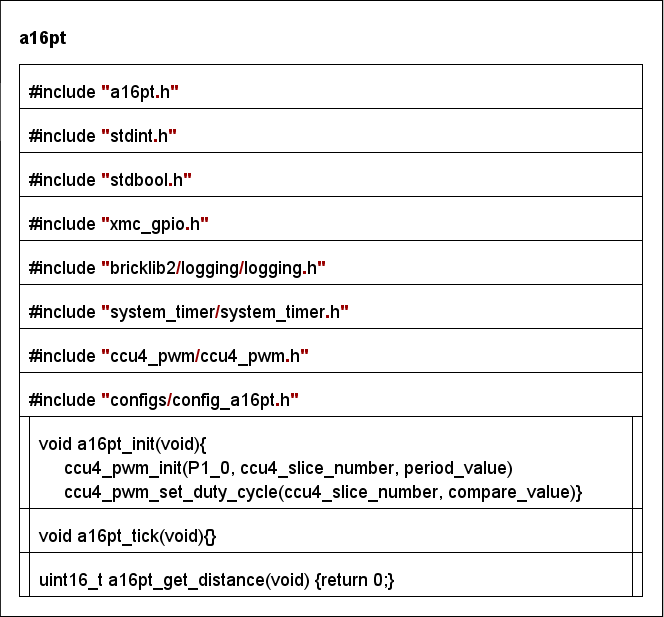
\includegraphics[width=1.0\textwidth]{Struktogramme/a16pt.png}\caption{Struktogramm der a16.pt}\label{fig:Bild2}
%\end{figure}


